%************************************************
\chapter{Graph Notation}
\label{chapter:graph_notation}
%************************************************

\section{Dynamic Activities as a Set}

\begin{figure}
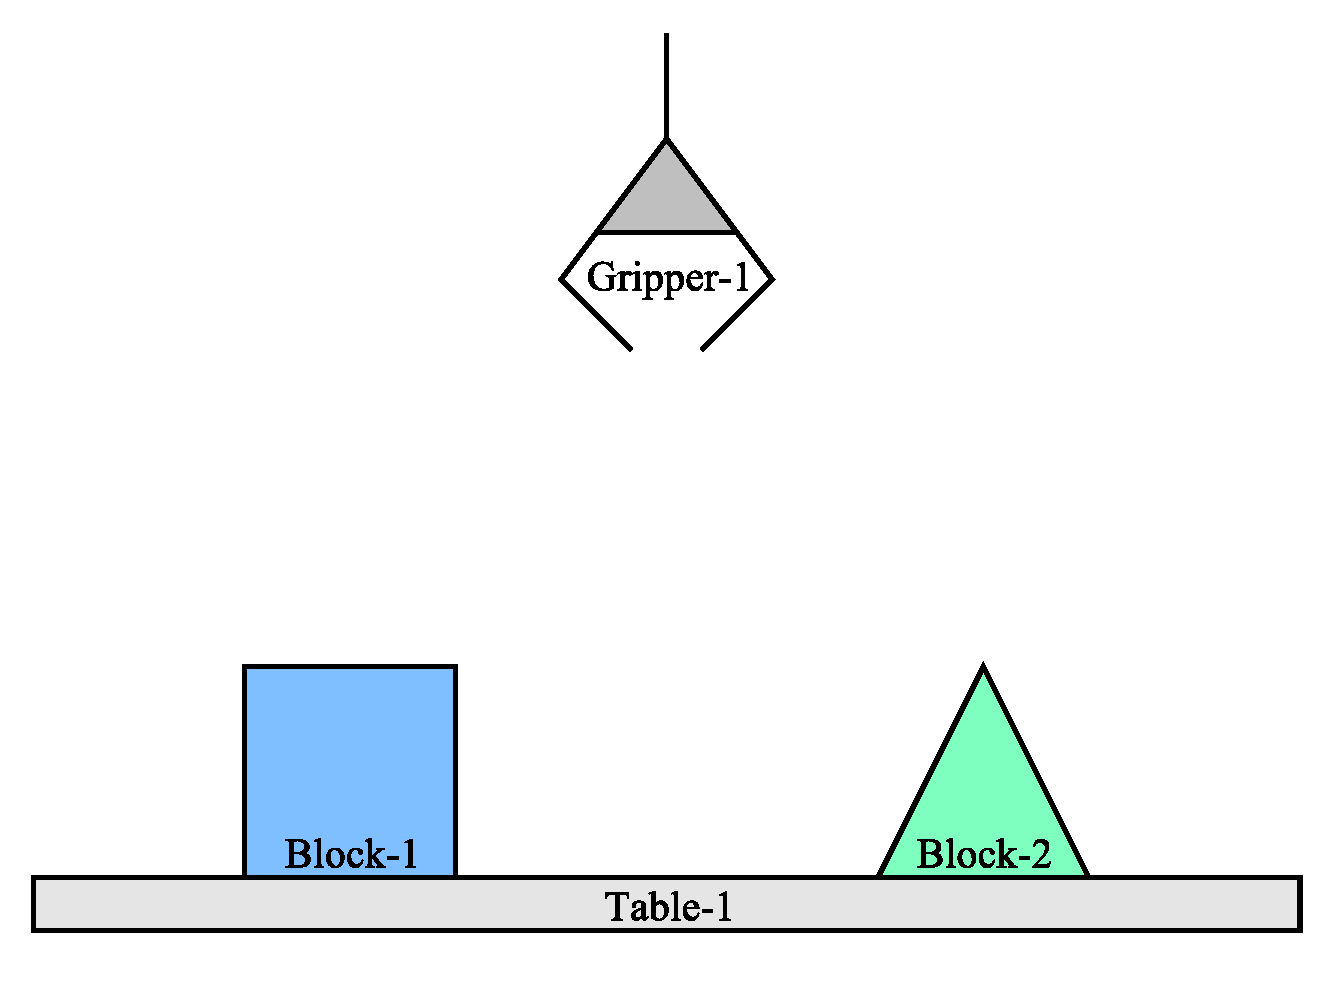
\includegraphics[width=10cm]{gfx/blocks_world_simulation}
\caption{An example for simulation.}
\label{figure:blocks_world_simulation}
\end{figure}

I will begin with one of the simplest mathematical models, a
\emph{set} of symbols, to model of the activities in Duration.  I will
first describe the simulation model as the mathematical set, X, the
activities of the state.  Here is an example of a possible
symbolization of the activities shown in
{\mbox{\autoref{figure:blocks_world_simulation}}}:
\begin{equation}
\label{equation:example_initial_state}
X =
  \left\{
    \begin{array}{l}
      \text{{\tt{Gripper-1}}}, \\
      \text{{\tt{Block-1}}}, \\
      \text{{\tt{Block-2}}}, \\
      \text{{\tt{Table-1}}} \\
      \text{{\tt{sitting-on}}}, \\
      \text{{\tt{being-above}}}, \\
      \text{{\tt{moving}}}, \\
      \text{{\tt{left}}}
    \end{array}
  \right\}
\end{equation}

\section{Representing Continuous Space as a Set of 3-Tuples}

The activities in Duration exist in a continuous Spatial arrangement
that is symbolized and ordered by the reflective thinking layers.  In
order to simulate this continuous homogenous Space, a discrete static
representation must be included in the state of the simulation model.
A 3-tuple can be used to represent the activity of a Spatial
relationship in the simulation.  Reconsidering the activities shown in
{\mbox{\autoref{figure:blocks_world_simulation}}}, the state could be
represented by the set of 3-tuples shown in
{\mbox{\autoref{equation:example_stricly_ordered_set_initial_state}}}.
\begin{equation}
\label{equation:example_stricly_ordered_set_initial_state}
\text{triples}(S) =
  \left\{
    \begin{array}{l}
      (\text{\tt{Block-1}},   ~\text{\tt{sitting-on}},  ~\text{\tt{Table-1}}), \\
      (\text{\tt{Block-2}},   ~\text{\tt{sitting-on}},  ~\text{\tt{Table-1}}), \\
      (\text{\tt{Gripper-1}}, ~\text{\tt{being-above}}, ~\text{\tt{Table-1}}), \\
      (\text{\tt{Gripper-1}}, ~\text{\tt{moving}},      ~\text{\tt{left}})
    \end{array}
  \right\}
\end{equation}

\section{A Graph Representation}

A set of 3-tuples can be thought of as a graph of nodes with labelled
edges.  Because the graph provides a clear notation for referring to
types of Spatial arrangements of activities, a modified notation
originally from {\mbox{\cite{messmer:1995}}} is used to define a
labelled graph in {\mbox{Definition~\ref{definition:graph_first}}} and
a labelled subgraph in
{\mbox{Definition~\ref{definition:graph_last}}}.

\begin{definition}
\label{definition:graph_first}
\emph{
A graph $G$ is the 3-tuple $(V, ~E, ~\mu)$, where
\begin{itemize}
\item $V$ is the set of vertices,
\item $E ~{\subseteq}~ V ~{\times}~ V$ is the set of edges,
\item $\mu : E \mapsto \{\ell_E\}$ is a function assigning a set of labels to each edge.
\end{itemize}
}\end{definition} \noindent In this definition, the edges are
directed, i.e. there is an edge from $v_1$ to $v_2$ if $(v_1,
v_2){\in}E$.  The empty graph, i.e. the graph with an empty set of
vertices will be denoted by $\emptyset$.  The union of the set of
vertices with the set of labels referred to by $\mu$ will be sometimes
be referred to with a dot notation, $\mathring{G}=V {\cup} \ell_E$.

\begin{definition}
\label{definition:graph_last}
\emph{ Given a graph $G = (V, E, \mu)$, a \emph{subgraph} of $G$ is a
  graph $G_s = (V_s, E_s, \mu_s)$ such that
\begin{enumerate}
\item $V_s ~{\subseteq}~ V$
\item $E_s ~{\subseteq}~ V_s {\times} V_s$,
\item $\mu_s$ is the restriction of $\mu$, i.e.
\begin{align*}
\mu_s(e) &\subseteq
   {\left\{
      \begin{array}{ll}
        \mu(e)     & \text{if }e {\in} E_s \\
        \text{undefined} & \text{otherwise}
      \end{array}
    \right.}
\end{align*}
\end{enumerate}
}\end{definition} \noindent From this definition it is easy to see
that, given a graph $G$, any subset of its vertices and an included
subset of its edges uniquely defines a subgraph of $G$.  The notation
$G_s ~{\subseteq}~ G$ is used to indicate that $G_s$ is a subgraph of
$G$.

\section{Representing Continuous Space as a Graph}

{\mbox{\autoref{figure:simulation_example_state}}} shows the example
simulation state state, initially presented in
{\mbox{\autoref{equation:example_stricly_ordered_set_initial_state}}},
as a set of 3-tuples, represented as a graph.  Graph notation will be
used to describe the activities in Duration and continuous Space,
which exist before they are symbolized and discretely ordered by the
$\text{reflective}^1$ layer.  The simulation model state space, $S$,
is defined to be a graph in
{\mbox{Equations~\ref{equation:define_graph_state_first}}}
{\mbox{through~\ref{equation:define_graph_state_last}}}.
\begin{align}
\label{equation:define_graph_state_first}
       S &= (S_V, ~S_E, ~S_\mu) \\
     S_V &= {\left\{
               \begin{array}{l}
                 \text{\tt{Gripper-1}}, \\
                 \text{\tt{Block-1}}, \\
                 \text{\tt{Block-2}}, \\
                 \text{\tt{Table-1}}, \\
                 \text{\tt{left}}
               \end{array}
             \right\}} \\
     S_E &= {\left\{
               \begin{array}{l}
                 (\text{\tt{Gripper-1}}, \text{\tt{Table-1}}), \\
                 (\text{\tt{Block-1}}, \text{\tt{Table-1}}), \\
                 (\text{\tt{Block-2}}, \text{\tt{Table-1}}), \\
                 (\text{\tt{Gripper-1}}, \text{\tt{left}})
               \end{array}
             \right\}} \\
\label{equation:define_graph_state_last}
S_\mu(e) &=
  {\left\{
     \begin{array}{ll}
       \{\text{\tt{being-above}}\} & \text{if }e = (\text{\tt{Gripper-1}}, \text{\tt{Table-1}}) \\
       \{\text{\tt{sitting-on}}\}  & \text{if }e = (\text{\tt{Block-1}}, \text{\tt{Table-1}}) ~{\vee}~ \\
                                   & \text{~~ }e = (\text{\tt{Block-2}}, \text{\tt{Table-1}}) \\
       \{\text{\tt{moving}}\}      & \text{if }e = (\text{\tt{Gripper-1}}, \text{\tt{left}}) \\
       \text{undefined} & \text{otherwise}
     \end{array}
   \right.}
\end{align}
\begin{figure}
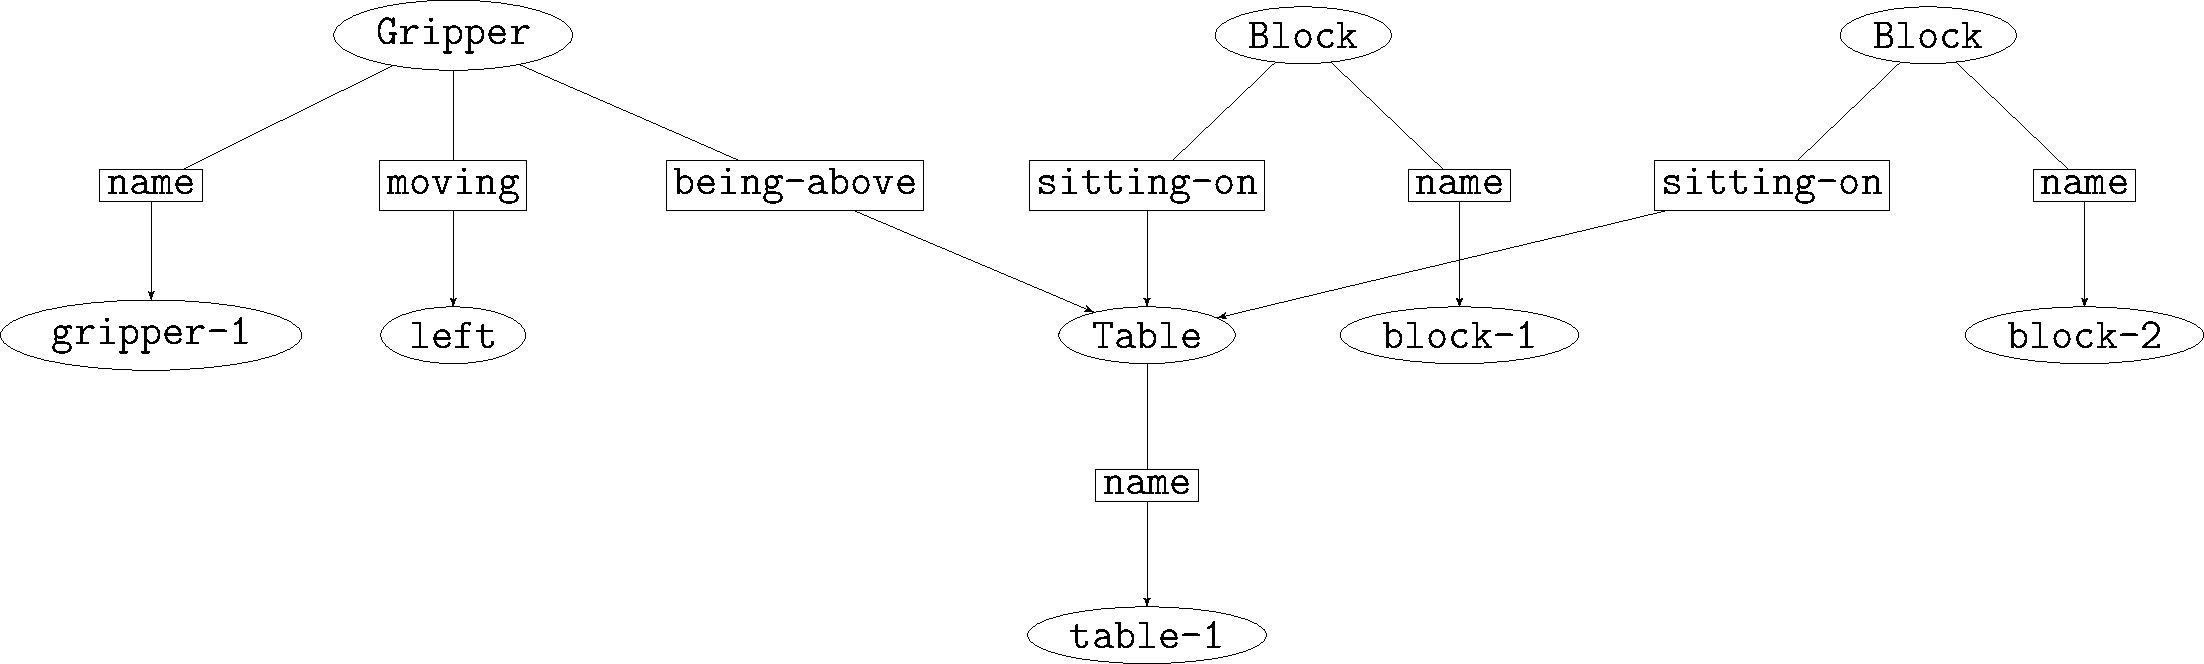
\includegraphics[width=10cm]{gfx/simulation_example_state}
\caption[A labelled graph representation of a state space.]{A labelled graph representation of a state space, where circles represent nodes, and squares represent edges.}
\label{figure:simulation_example_state}
\end{figure}

\section{Dot Notation for Graph-based Frame Objects}

Sometimes it is useful to refer to parts of a graph by considering
nodes in the graph to represent frame objects that have slotted
relationships with other frame objects.  Thus, I use a dot notation to
refer to the set of nodes that are connected to a given node, $v_1$,
through a given edge label, $\ell_e$, as defined in
{\mbox{\autoref{equation:frame_dot_notation}}}.
\begin{equation}
\label{equation:frame_dot_notation}
v_1.\ell_e = \{v_2 ~:~ (v_1, v_2) \in S_E \wedge \ell_e \in \mu[(v_1, v_2)]\}
\end{equation}

\section{Simulated Existence}

Activities in continuous Space actually exist.  Once we have
considered the activities in Duration to be the set of symbols, $S$,
we have assumed static representations for the actual dynamic.  The
dynamic does not have terms to help us in representing.  Therefore,
the question of existence becomes a question of whether or not a
symbol is in the set that is the current state of the simulation, $S$.
Equation~\ref{equation:exists} shows a definition of {\tt exists},
defined as the subgraph relationship between any state, $x$,
represented as a labelled graph, and the currently simulated state
graph, $S$:
\begin{equation}
\label{equation:exists}
\text{exists}(x) \longleftrightarrow x ~{\subseteq}~ S
\end{equation}

\section{Representing Reflective Thinking Activity}

Reflective thinking exists as activities in Duration alongside the
physical activities that have just been described.  I will refer to
the subgraph that represents the $\text{reflective}^1$ thinking
activities as $\mathcal{R}^1$.  The first symbolic reference to
reflective thinking is now introduced to this layer of the model.
Note that I have not introduced any specific symbolic physical
activity to the model.  The block example is just that, an example.
Having no symbolic references in the physical layer of the simulation
is important for keeping the representation for the reflective focus
as any labelled graph, which subsequently allows for reflection over
itself, whatever the specific graph representation of reflective
thinking that will now be described.  This is a key point.

I will use the symbol {\tt $\text{reflective}^1$} to refer to the
activity of the first-order reflective layer.  This symbol is grounded
in the activity in Duration that currently actually exists.  This
symbol does not refer the simulated activities in Duration in the
simulation model.  This symbol is grounded in the understanding of the
model of mind.  The reflective activity is primarily reflecting on the
rest of the simulation state, everything that existed before the
$\text{\tt{reflective}}^1$ node was added to the simulation state
graph.

\section{Physical Activity is Any Prior Existing Graph}

Prior to this symbol existing in the simulation state graph, there
have been no other specific symbols introduced.  This graph of
physical activities must necessarily exist prior to reflectively
thinking about it.  Because this prior activity is defined to be
\emph{any} graph, what remains in order to build $n$ layers of
reflective thinking activity is to define a reflective planning
activity that reflects upon this prior activity.  Therefore,
subsequently, no matter what the reflective thinking description, this
reflective thinking activity can be duplicated in $n$ reflective
layers that will reflectively think about any given graph
representation of activity.  Allowing the physical activity to a be an
undescribed graph is important in order to allow this recursion.
Notice that the physical activity is not necessarily composed of
anything resembling objects as graphs are a very general
representation that could just as easily represent one single number
line, or even an infinitely finely interpolated multidimensional
Space.  If some prior physical activity can be represented as a graph,
then this simulation of reflective thinking is equally applicable.

\section{Defining N Layers of Reflective Thinking Activities}

Layers of reflective activity are defined inductively, beginning with
$\text{reflective}^0$ layer of activity, $\mathcal{R}^0$, as the
initial given physical activity, $\mathcal{P}$.  Then, each subsequent
layer of $\text{reflective}^{n+1}$ thinking activity,
$\mathcal{R}^{n+1}$, is defined in terms of $\mathcal{R}^n$ in
{\mbox{Equations~\ref{equation:define_reflective_n_activity_graph_first}}}
{\mbox{through~\ref{equation:define_reflective_n_activity_graph_last}}}.
\begin{align}
\label{equation:define_reflective_n_activity_graph_first}
                                        \mathcal{R}^0 &= \mathcal{P} \\
                                     \mathcal{R}^{n+1}_V &\subset S_V \setminus \bigcup_{k=0}^n\mathcal{R}^k_V \\
                                   \mathcal{R}^{n+1}_E &= (\mathcal{R}^{n+1}_V \times \mathcal{R}^{n+1}_V) \cap S_E \\
\label{equation:define_reflective_n_activity_graph_last}
                              \mathcal{R}^{n+1}_\mu(e) &= {\left\{
                                                            \begin{array}{ll}
                                                              S_\mu(e)          & \text{if }e {\in} \mathcal{R}^{n+1}_E \\
                                                              \text{undefined} & \text{otherwise}
                                                            \end{array}
                                                          \right.}
\end{align}

\section{Representing a Graph in the State}

One of the basic capabilities of the reflective simulation is the
ability to create a reference, $x$, to an arbitrary subgraph of
activity, $\Psi(x)$, in the simulation state, $S$.
{\mbox{Equations~\ref{equation:first_order_reflection_representation_in_state_first}}}
{\mbox{through~\ref{equation:first_order_reflection_representation_in_state_last}}}
show a definition of a graph representation within the state graph.
\begin{align}
\label{equation:first_order_reflection_representation_in_state_first}
                                                                    \Psi(x) &\subset S \\
                                                         x.\text{\tt{node}} &= \Psi_V(x) \\
                                               \forall e \in \Psi_E(x), x_e &\in x.\text{\tt{edge}} \\
   \forall_{e \in \Psi_E(x)}, e = (e_{v_1}, e_{v_2}) \wedge x_e.\text{\tt{tail}} &= \{e_{v_1}\} \\
   \forall_{e \in \Psi_E(x)}, e = (e_{v_1}, e_{v_2}) \wedge x_e.\text{\tt{head}} &= \{e_{v_2}\} \\
\label{equation:first_order_reflection_representation_in_state_last}
                              \forall_{e \in \Psi_E(x)}, x_e.\text{\tt{label}} &= \Psi_\rho(x)(e)
\end{align}

\section{Representing the Reflective Focus}

Once there is given physical activity defined in the state graph, $S$,
the first-order reflective activity is a dynamic reference to this
given activity.  Here, I introduce the first symbolic references to
this dynamic first-order reflective activity,
$\text{\tt{reflective}}^n$.
{\mbox{Equations~\ref{equation:reflective_symbol_in_state_first}}}
{\mbox{and~\ref{equation:reflective_symbol_in_state_last}}} define the
reflective focus on the given activity.
\begin{align}
\label{equation:reflective_symbol_in_state_first}
        \text{\tt{reflective}}^n &\in \mathcal{R}^n_V, \text{~for $n \geq 1$} \\
\label{equation:reflective_symbol_in_state_last}
  \Psi(\text{\tt{reflective}}^n) &\subset S \setminus \bigcup_{k=n}^\infty\mathcal{R}^k_V
\end{align}
{\mbox{\autoref{figure:simulation_reflective_1_example_state}}} shows
how the $\text{\tt reflective}^1$ symbolic dynamic activity is in a
continuous Spatial arrangement with the physical layer of activities.
\begin{figure}
\center
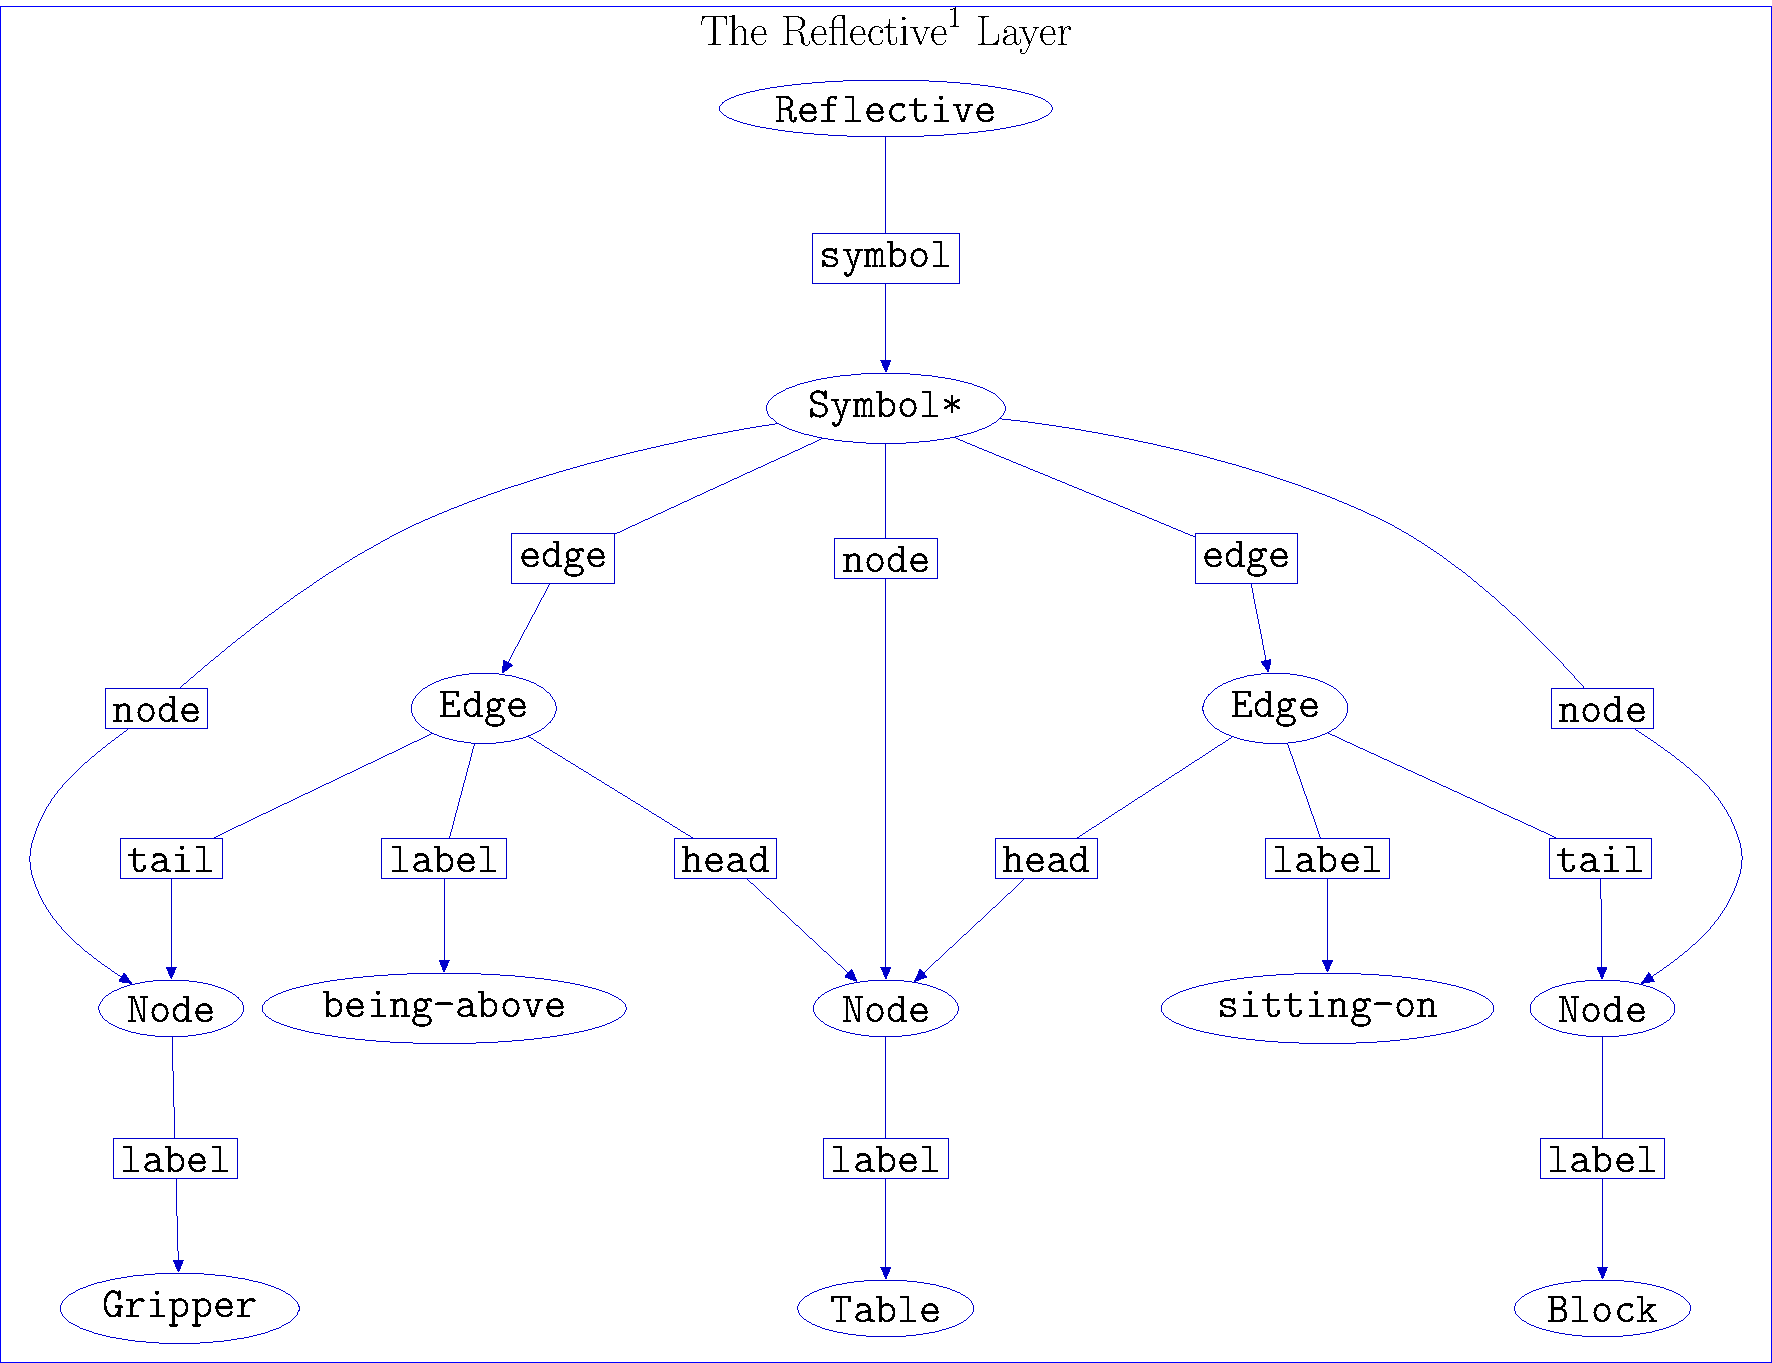
\includegraphics[width=12cm]{gfx/simulation_reflective_1_example_state}
\caption[The $\text{\tt reflective}^1$ activity focused on physical
  activity.]{The $\text{\tt reflective}^1$ activity focused on
  $\text{reflective}^0$ activity, where black and blue colors
  distinguish $\text{reflective}^0$ and $\text{reflective}^1$ layers
  of Spatial arrangements of activities, respectively.}
\label{figure:simulation_reflective_1_example_state}
\end{figure}

\section{A Visualization of a Reflective Relationship}

When reflective graph structures, as in
{\mbox{\autoref{figure:simulation_reflective_1_example_state}}}, get
to be larger, they can be confusing when shown in full structural
detail.  In order to simplify the visual representation of a
reflective relationship, I will sometimes use a trapezoidal edge-like
visual in order to present the same complicated relationship structure
in a simpler way.
{\mbox{\autoref{figure:reflective_relationship_visualization}}} shows
a simpler visualization of the same example reflective relationship.
\begin{figure}
\center
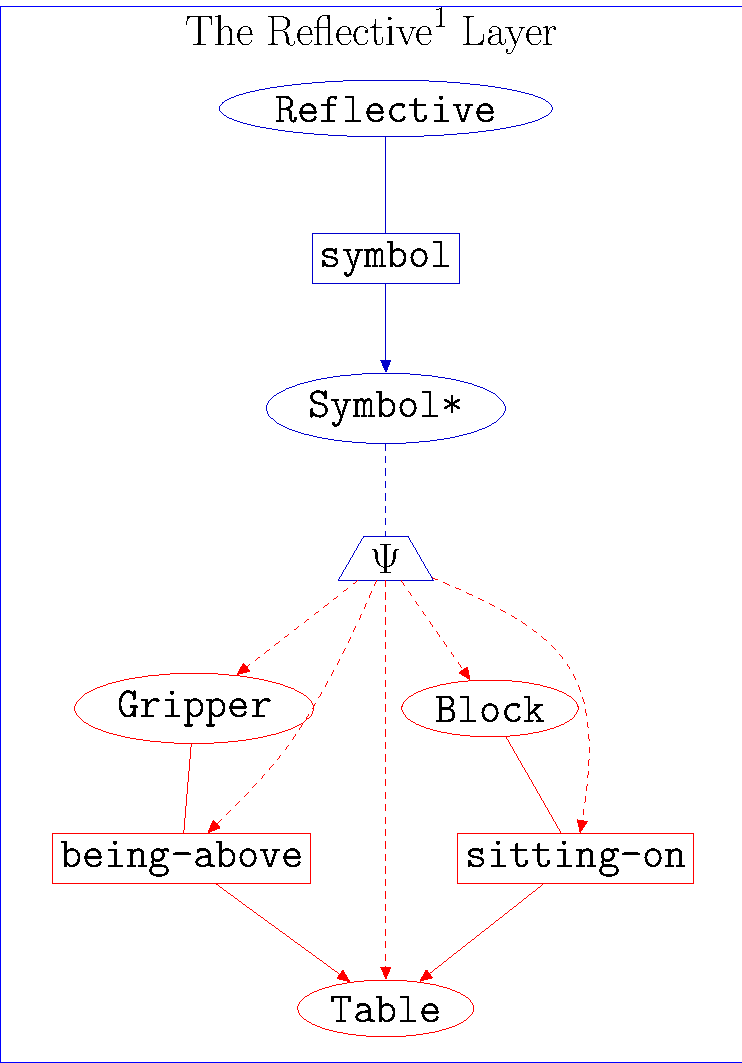
\includegraphics[width=8cm]{gfx/reflective_relationship_visualization}
\caption[A reflective relationship visualization.]{A reflective
  relationship visualization, where the trapezoid is a visual
  representation, a shorthand, for the same reflective relationship
  depicted in
  {\mbox{\autoref{figure:simulation_reflective_1_example_state}}}.
  Note that the subgraph, $\Psi$, of the state graph, $S$, is not
  itself a symbol in the state graph.}
\label{figure:reflective_relationship_visualization}
\end{figure}

\section{Representing Symbolic Reference}

In order to describe symbolization, a representation for a simulated
symbol must be defined.  A symbol is the most interesting object in
the model because it functions as a static reference to the dynamic,
while being fundamentally dynamic itself.  There are two primary
features of a symbolic reference:
\begin{itemize}
\item A symbol functions as a static reference and, thus, can be
  ordered in Spatial arrangements that function as static orderings.
\item A symbol is fundamentally dynamic and, thus, exists as dynamic
  activities in a referential dynamic continuous Spatial relationship
  with other dynamic activities in Duration.
\end{itemize}
A symbol is actively maintained in Duration, so the existence of a
simulated symbol in the simulation model would need to be added to the
set of all simulated activities in Duration.  The set of symbols* in
layer $n$ is defined to be $X^{*n}$.
{\mbox{Equations~\ref{equation:define_symbol_first}}}
{\mbox{and~\ref{equation:define_symbol_last}}} define layered sets of
symbols*:
\begin{align}
\label{equation:define_symbol_first}
           X^{*n} &= \text{\tt{reflective}}^n.\text{\tt{symbol}} \\
\label{equation:define_symbol_last}
           x^{*n} &\in X^{*n}
\end{align}
Each symbol*, $x^{*n}$, has a reflective focus, $\Psi(x^{*n})$, a
subgraph of the simulated activities in Duration, $S$.
{\mbox{Equation~\ref{equation:define_symbol_referent_graph}}} defines
the referent subgraph, $\Psi(x^{*n})$, for a symbol*, $x^{*n}$:
\begin{equation}
\label{equation:define_symbol_referent_graph}
  \Psi(x^{*n}) \subseteq X^{*n} \cup \bigcup_{k=0}^{n-1}\mathcal{R}^k_V
\end{equation}

\section{Representing Symbolic Perception and Memory}

{\mbox{\autoref{figure:example_symbolic_reference_to_physical_activity}}}
shows an example of a symbol*, $x_1^*$, in the first-order reflective
layer.  Notice that $\Psi(x_1^*)$ is a subgraph of
$\Psi(\text{\tt{reflective}}^1)$.  When a symbolic reflective
reference is contained within the reflective focus, the symbol is said
to be a \emph{symbolic perception}.
{\mbox{\autoref{figure:example_symbolic_memory}}} shows a symbolic
reflective reference, $x_2^*$, to the physical layer of activity that
is not perceived because it is not contained within the first-order
reflective focus.  When a symbol is not contained within the
reflective focus, this is referred to as a \emph{symbolic memory}.
Note that the physical, $\text{reflective}^0$ layer of activity
includes all physical activity, including not only current symbolic
perceptions but also symbolic memories.  In this sense, as the AI
changes reflective focus, the perceived dynamic physical activity
changes.
\begin{figure}
\center
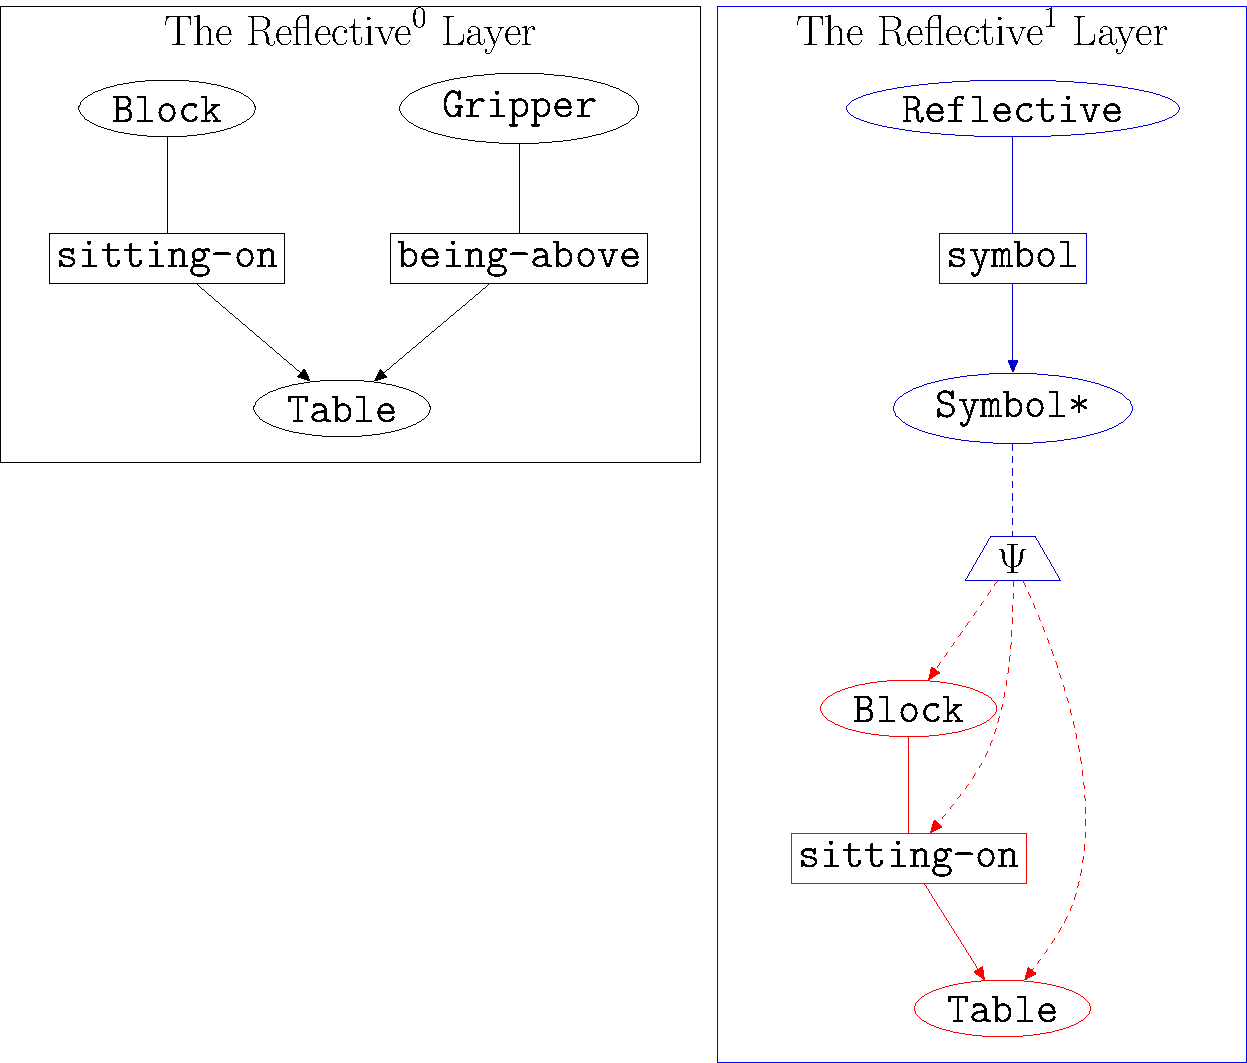
\includegraphics[height=10cm]{gfx/example_symbolic_reference_to_physical_activity}
\caption{Example of a perceived first-order symbolic reference to the
  physical layer of activity,
  i.e. $\Psi(x_1^*)\subseteq\Psi(\text{\tt{reflective}}^1)$.}
\label{figure:example_symbolic_reference_to_physical_activity}
\end{figure}
\begin{figure}
\center
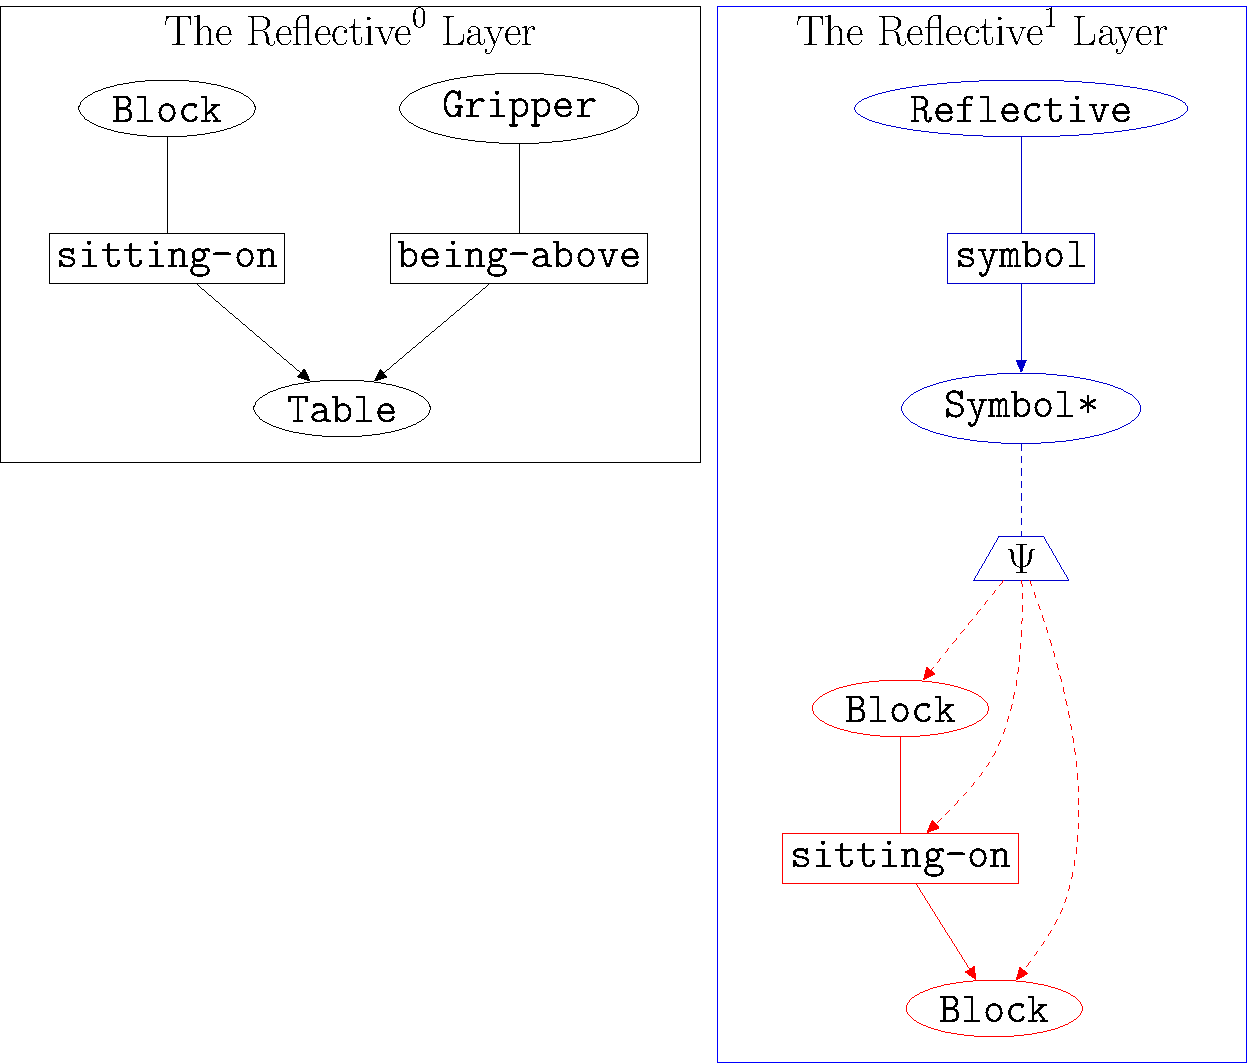
\includegraphics[height=10cm]{gfx/example_symbolic_memory}
\caption{Example of a non-perceived symbol, or symbolic memory,
  i.e. $\Psi(x_2^*)\not\subseteq\Psi(\text{\tt{reflective}}^1)$.}
\label{figure:example_symbolic_memory}
\end{figure}

\section{Representing Static Space}

Spatial arrangements of static symbols are created by the reflective
thinking layers.  Static symbols are not contained within the physical
layer, but these symbols are used to represent transitions from the
past to the future, which are in turn used to create relationships
between causes and effects that are used for planning.  Thinking
activities use these Spatial arrangements of symbols to think about
the given activities of the physical layer as well as planning in the
first-order reflective layer.

\section{Representing Simultaneities and Transitions}

As {\mbox{\autoref{equation:define_symbol_referent_graph}}} states,
each reflective thinking layer can create static symbolic references
to activities in the layers below as well as any static symbolic
activities in or below that layer.  Simultaneities and transitions are
the basis for representing concurrent and sequential event knowledge.
It is a type of static Spatial arrangement between static symbolic
references.  Simultaneities and transitions can be arranged into
sequences back in time, forward in time, as well as organizing time
into binary trees for efficient recall.
\begin{figure}
\center
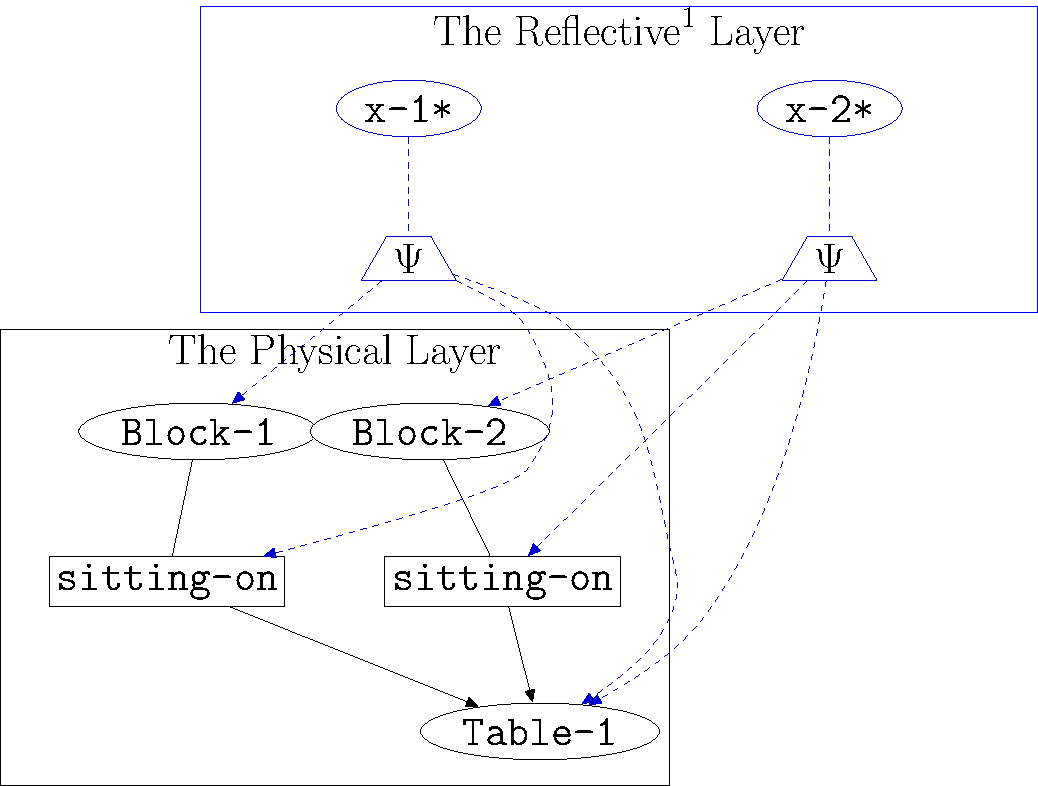
\includegraphics[width=10cm]{gfx/two_example_grounded_symbolic_references}
\caption[Two example symbolic references.]{Two example grounded symbolic references, $x_1^*$ and $x_2^*$.}
\label{figure:two_example_grounded_symbolic_references}
\end{figure}
\begin{figure}
\center
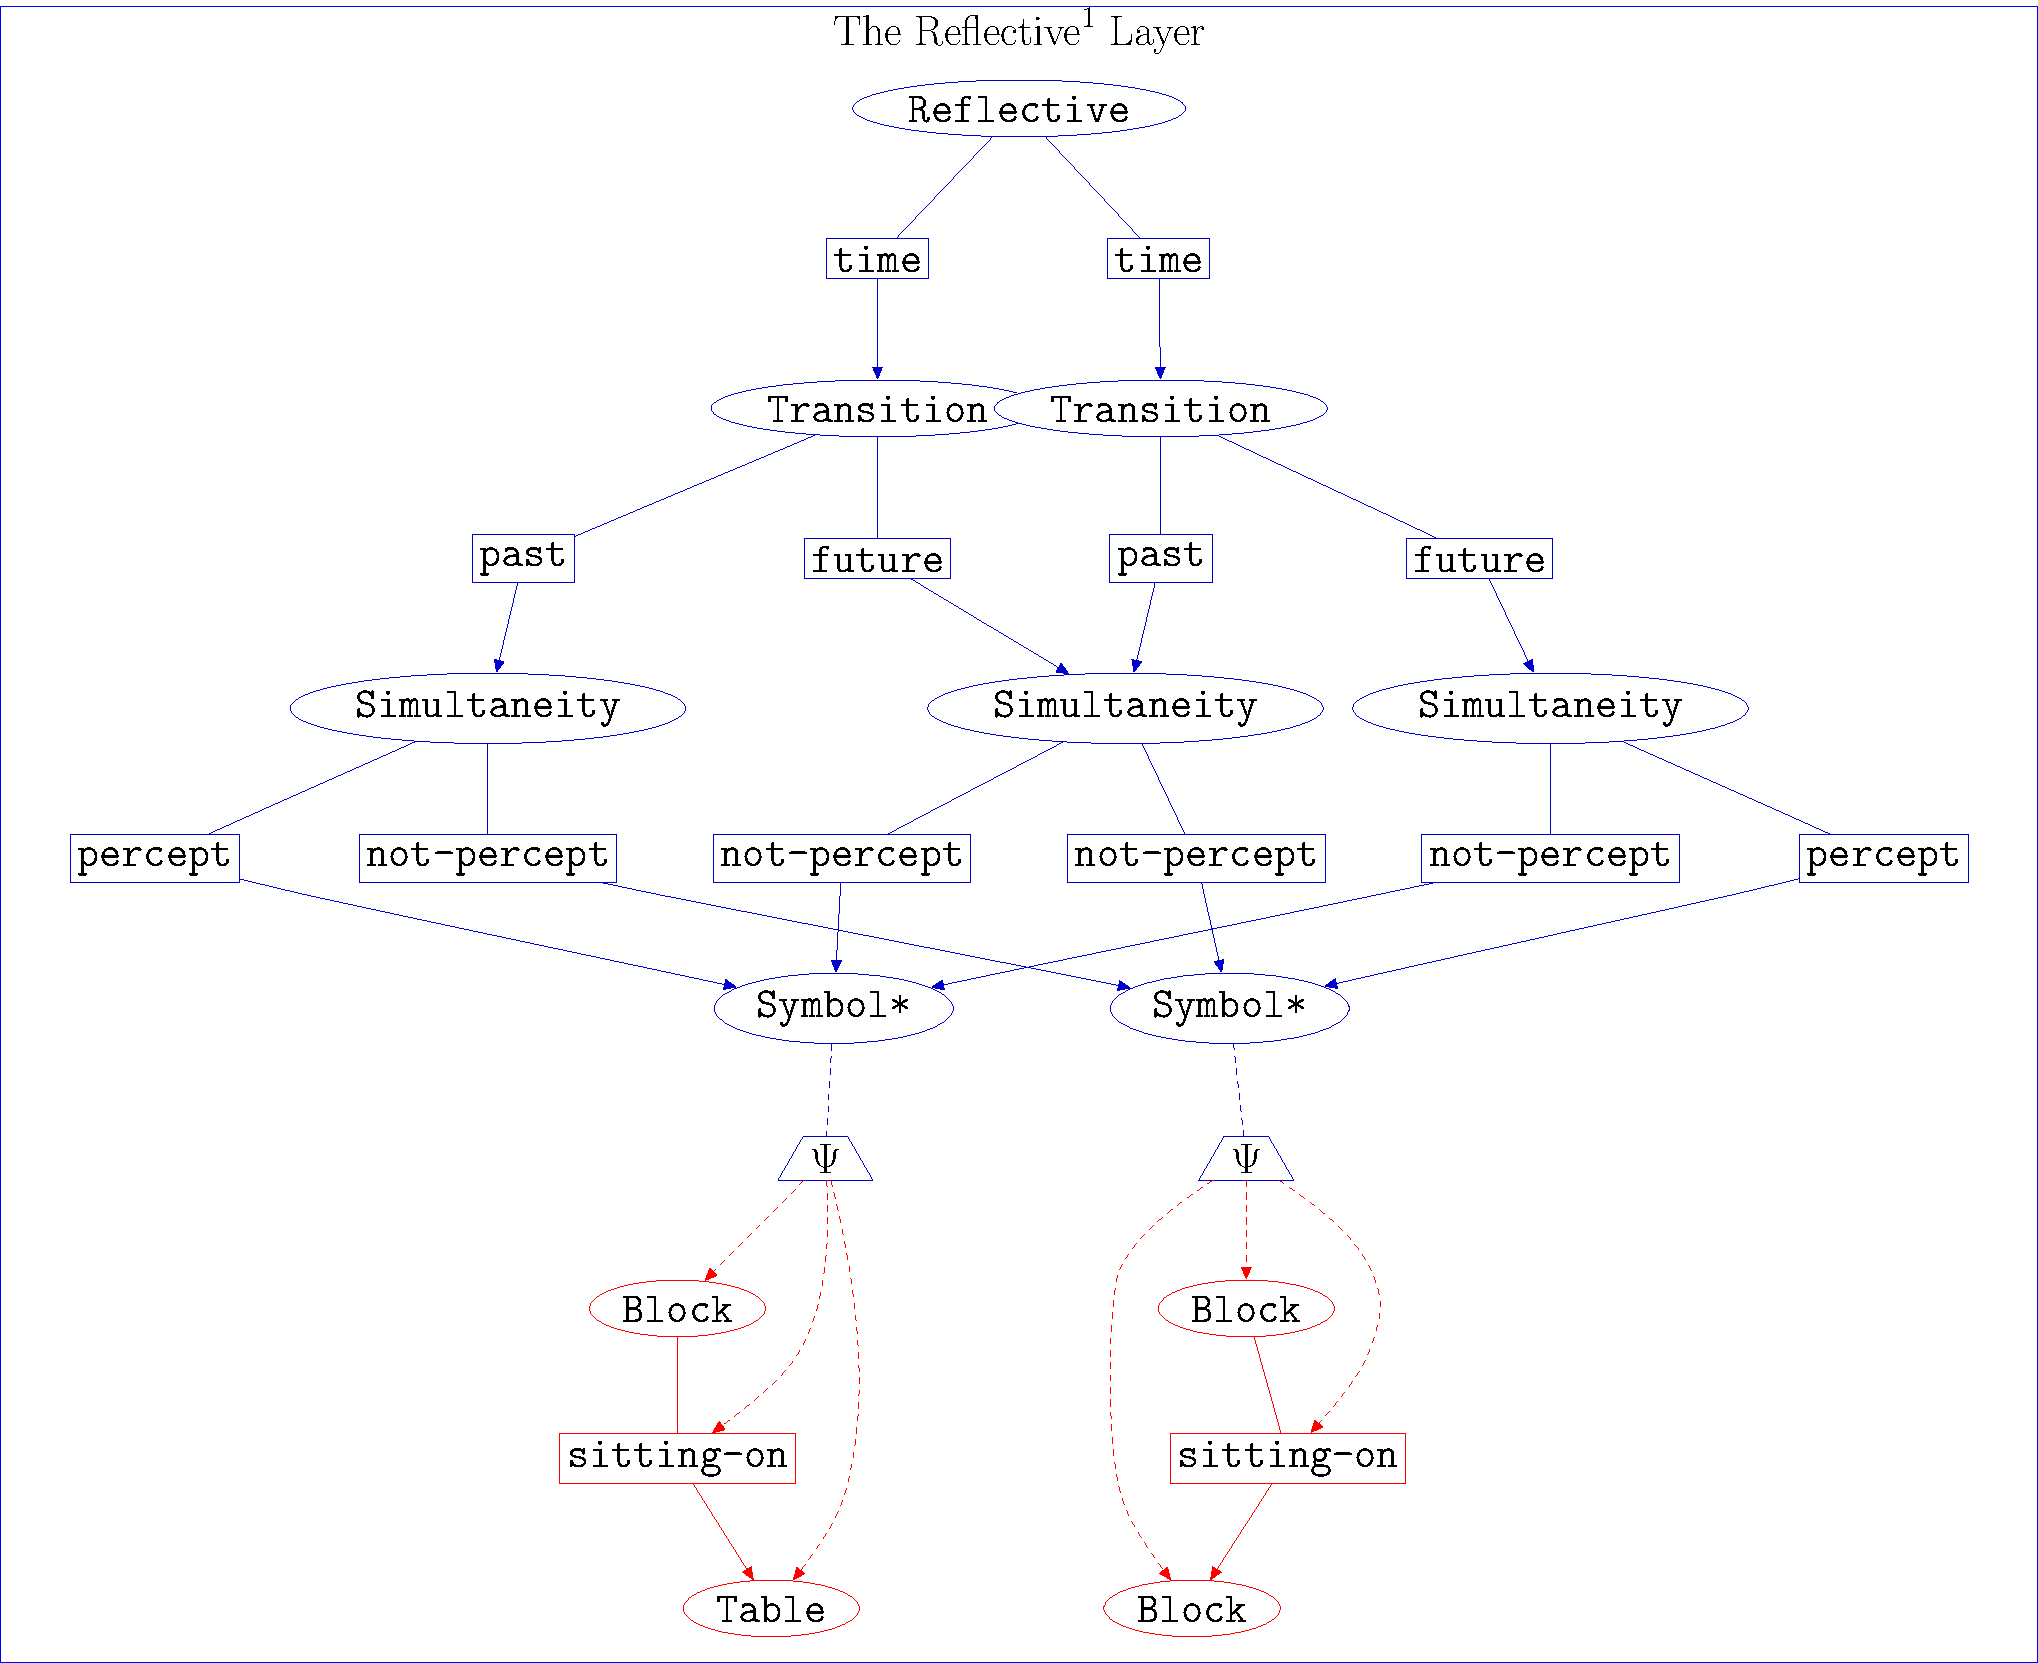
\includegraphics[width=10cm]{gfx/example_transition}
\caption[An example of a transition between simultaneities.]{An
  example of a transition between simultaneities of first-order static
  symbolic references, $x_1^*$ and $x_2^*$.}
\label{figure:example_transition}
\end{figure}










\section{leftovers...}

\section{Tautological Symbolic Reference}

{\mbox{Equations~\ref{equation:tautological_reference_first}}}
{\mbox{through~\ref{equation:tautological_reference_last}}} give an
example of a symbol*, $x^*$, that tautologically references its own
symbolization activity:
\begin{align}
\label{equation:tautological_reference_first}
\rho(x^*) &= (V_x, ~E_x, ~\mu_x, ~\nu_x) \\
 V_{x^*}   &= \{v_1\} \\
 E_{x^*}   &= \emptyset \\
 \mu_{x^*} &= v : \{v_1\} ~{\mapsto}~ \{x^*\} \\
\label{equation:tautological_reference_last}
            \nu_{x^*} &= e : \emptyset ~{\mapsto}~ \emptyset
\end{align}
Tautological references are meaningless.  In a model that is
symbolizing and perceiving the world in terms of symbols, tautological
symbolic references always have the potential for being active
perceptions because the existence of a tautological symbol implies
that its referent, itself, is active.  When symbols are used for
perception, tautological references are at best distracting and at
worst render a model meaningless.

Because a tautological reference removes all utility from symbols* in
the simulation model, it is important that avoiding tautological
references is the default behavior.  In order to easily avoid
tautological references, I define an ordering for symbolic references
that keeps references from ever becoming purely tautological.




\section{leftovers...}

\section{Simulation States}

At any given point in the simulation, the state, $S$, is static, but
the simulation can have different static states at different time
steps, $n$, giving a number of static states, $S[n]$.  The simulation
process is a discrete stepwise activity.  The simulation step is the
dynamic activity that is not part of the state, $S$, of the simulation
model.  I will now describe a notation for referring to the different
states that result from a simulation process.

Equations~\ref{equation:simulate_first}
and~\ref{equation:simulate_last} show a notation for referring to the
state of a simulation after a number of simulation steps, $n$.
\begin{align}
\label{equation:simulate_first}
S[0] &= \text{\emph{The Initial State}} \\
\label{equation:simulate_last}
S[n] &= \text{\emph{simulate}}~S[n-1]
\end{align}
Equation~\ref{equation:simulate_first} defines $S[0]$ to be
the initial representation of the activities in Duration that are
being simulated; an example of the initial state was given previously
in Equation~\ref{equation:example_initial_state}.
Equation~\ref{equation:simulate_last} introduces an explicit reference
to the activity of simulation with the symbol ``simulate.''  Because I
have not yet defined this activity, these equations still have a
reference to the actual dynamic activity of simulation.  I use this
notation to discuss how the state, $S$, changes during the
actual process of simulation.  I will use the notation in
Equation~\ref{equation:simulate_n_steps} to refer to the state of the
simulation after $n$ actual steps of simulation activity:
\begin{equation}
\label{equation:simulate_n_steps}
S[n] = \text{\emph{simulate}}^n~S[0]
\end{equation}



% Original definition of a graph as a 4-tuple with labelled nodes and edges

%\begin{definition}
%\label{definition:graph_first}
%\emph{
%A graph $G$ is the 4-tuple $(V, ~E, ~\mu, ~\nu)$, where
%\begin{itemize}
%\item $V$ is the set of vertices,
%\item $E ~{\subseteq}~ V ~{\times}~ V$ is the set of edges,
%\item $\mu : V \mapsto \ell_V$ is a function assigning a label to each vertex,
%\item $\nu : E \mapsto \{\ell_E\}$ is a function assigning a set of labels to each edge.
%\end{itemize}
%}\end{definition} \noindent In this definition, the edges are
%directed, i.e. there is an edge from $v_1$ to $v_2$ if $(v_1,
%v_2){\in}E$.  The empty graph, i.e. the graph with an empty set of
%vertices will be denoted by $\emptyset$.  The union of the sets of
%labels referred to by $\mu$ and $\nu$ will be sometimes be referred to
%with a dot notation, $\mathring{G}=\ell_V {\cup} \ell_E$.
%
%\begin{definition}
%\label{definition:graph_last}
%\emph{ Given a graph $G = (V, e, \mu, \nu)$, a \emph{subgraph} of $G$
%  is a graph $G_s = (V_s, e_s, \mu_s, \nu_s)$ such that
%\begin{enumerate}
%\item $V_s ~{\subseteq}~ V$
%\item $E_s ~{\subseteq}~ V_s {\times} V_s$,
%\item $\mu_s$ and $\nu_s$ are the restrictions of $\mu$ and $\nu$,
%  respectively, i.e.
%\begin{align*}
%\mu_s(v) &=         {\left\{
%                       \begin{array}{ll}
%                         \mu(v)           & \text{if }v {\in} V_s \\
%                         \text{undefined} & \text{otherwise}
%                       \end{array}
%                     \right.} \\
%\nu_s(e) &\subseteq {\left\{
%                       \begin{array}{ll}
%                        \nu(e)           & \text{if }e {\in} E_s \\
%                        \text{undefined} & \text{otherwise}
%                       \end{array}
%                     \right.}
%\end{align*}
%\end{enumerate}
%}\end{definition}



%\section{Simulating the Plan}
%


%\section{State Transitions (should be rewritten in simulation objects)} 

%\autoref{figure:blocks_world_gripper_over_block} shows an example of
%the next state of the simulation, $S[1]$.
%Equation~\ref{equation:example_next_state} gives an example
%description of the next state of the simulation model:
%\begin{figure}[bth]
%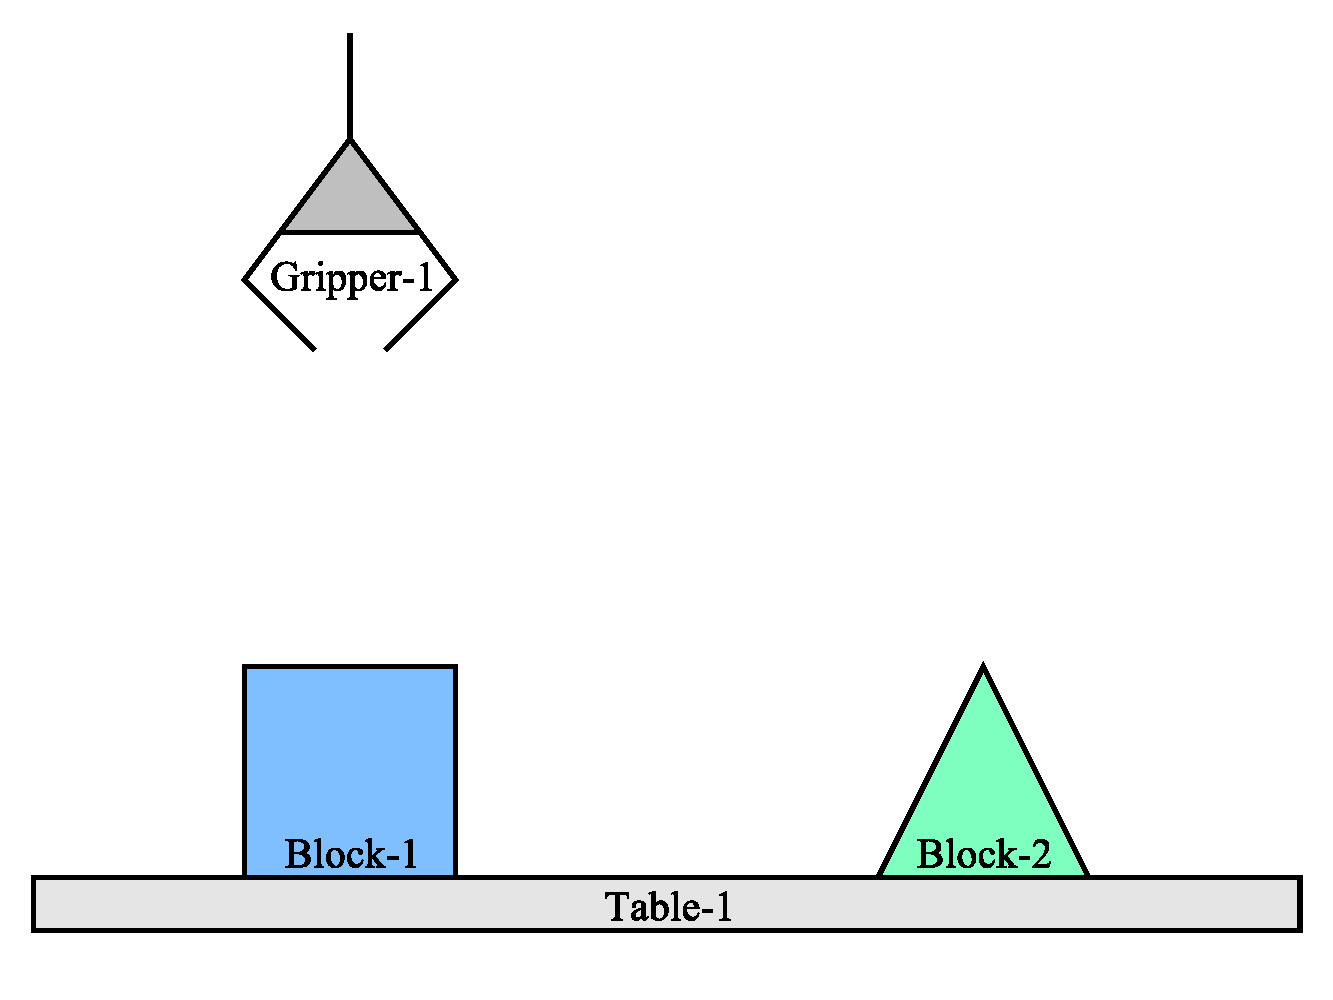
\includegraphics[width=10cm]{gfx/blocks_world_gripper_over_block}
%\caption{An example future state of simulation.}
%\label{figure:blocks_world_gripper_over_block}
%\end{figure}
%\begin{equation}
%\label{equation:example_next_state}
%S[1] =
%  \left\{
%    \begin{array}{l}
%      \text{{\tt Block-1-sitting-on-Table-1}}, \\
%      \text{{\tt Block-2-sitting-on-Table-1}}, \\
%      \text{{\tt Gripper-1-hovering-above-Table-1}}, \\
%      \text{{\tt Gripper-1-hovering-above-Block-1}}
%    \end{array}
%  \right\}
%\end{equation}
%
%Now, in order to begin to describe the activity of simulation, we must
%explicitly represent the transition, $T$, from one state to another.
%I refer to the resulting change to the state of the simulation as a
%\emph{state transition}.  The transition, $T[n]$, consists of two sets
%that keep track of changes, the \emph{add} set and the \emph{remove}
%set, as shown in Equation~\ref{equation:state_transition}:
%\begin{equation}
%\label{equation:state_transition}
%T[n] = \{T_\text{add}[n], ~T_\text{remove}[n]\}
%\end{equation}
%Equations~\ref{equation:predictive_state_transition}
%through~\ref{equation:transframe_last} give a definition of the
%transition, $T[n]$, in terms of the states, $S[n]$ and
%$S[n+1]$:
%\begin{align}
%\label{equation:predictive_state_transition}
%          S[n+1] & = S[n] ~{\cup}~ T_\text{add}[n] ~{\setminus}~ T_\text{remove}[n] \\
%         T_\text{remove}[n] & ~{\subseteq}~ S[n] \\
%         T_\text{remove}[n] & ~{\not\subseteq}~ S[n+1] \\
%            T_\text{add}[n] & ~{\subseteq}~ S[n+1] \\
%\label{equation:transframe_last}
%            T_\text{add}[n] & ~{\not\subseteq}~ S[n]
%\end{align}
%Equations~\ref{equation:state_transition_first}
%and~\ref{equation:state_transition_last} give the state transition,
%$T[n]$, for every step of the simulation:
%\begin{align}
%  \label{equation:state_transition_first}
%     T_\text{add}[n] &= S[n+1] ~{\setminus}~ S[n] \\
%  \label{equation:state_transition_last}
%  T_\text{remove}[n] &= S[n]   ~{\setminus}~ S[n+1]
%\end{align}
%Equation~\ref{equation:predictive_state_transition} shows the
%predictive potential for knowing the transition, $T[n]$, given the
%current state, $S[n]$.  Of course, $T[n]$ is defined in
%terms of $S[n]$ \emph{and} $S[n+1]$, so any
%predictive potential for
%Equation~\ref{equation:predictive_state_transition} is purely
%hypothetical.

